\documentclass[10pt]{beamer}

\usepackage[czech]{babel}
\usepackage{times}
\usepackage[utf8]{inputenc}
\usepackage[IL2]{fontenc}
\usepackage{algorithmic}
\usepackage[ruled,czech,linesnumbered]{algorithm2e}
\usepackage{hyperref}


\usetheme[progressbar=frametitle]{metropolis}
\setbeamertemplate{frame numbering}[fraction]
\useoutertheme{metropolis}
\useinnertheme{metropolis}
\usefonttheme{metropolis}
\definecolor{darklavender}{rgb}{0.45, 0.31, 0.59}
\setbeamercolor{background canvas}{bg=white}
\setbeamercolor{frametitle}{bg=darklavender}
\setbeamercolor{palette primary}{bg=darklavender}


\title[Short title]{\huge Binární vyhledávací strom}
\author{\Large Aleksandr Shevchenko}
\institute{\small Vysoké učení technické v Brně\\
    Fakulta informačních technologií}
\date{\today}

\begin{document}
\metroset{block=fill}

\begin{frame}
    \titlepage
\end{frame}

\begin{frame}{Obsah prezentace}
    \begin{enumerate}
    \item Motivace
    \item Binární vyhledávací strom
    \item Vyhledávání klíče
    \item Vložení klíče
    \item Smazání klíče
    \item Pseudokód BST
    \item Složitost BST, závěr
    \item Použité zdroje
    \end{enumerate}
\end{frame}

\begin{frame}[t]{Motivace}
    \smallskip
    \begin{block}{Proč potřebujeme řadicí algoritmy?}
    \medskip
    Pro rychlé vyhledávání a představu dat. Některé úlohy jsou nevyřešitelné bez zařazování.
    \end{block}
    \bigskip
    \bigskip
    \begin{columns}[onlytextwidth]
    \column{0.55\textwidth}
    \only<2->{
    \textbf{Některé populární algoritmy:}
    \begin{itemize}
    \item Bubble sort
    \item Shakesort
    \item Quicksort
    \item Radix sort
    \item Binary search tree
    \end{itemize}
    \column{0.45\textwidth}
    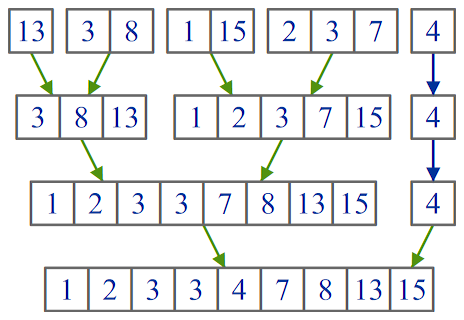
\includegraphics[scale=0.29]{radici.png}
    }
    \end{columns}
\end{frame}

\begin{frame}[t]{Binární vyhledávací strom}
    \smallskip
    \begin{block}{Definice}
    \medskip
    \textbf{Binární vyhledávací strom} (Binary Search Tree\,--\,BST) je datová struktura založená na binárním stromu, umožňující rychlé vyhledávání daných hodnot.
    \end{block}
    \medskip
    Základní vlastnosti:
    \begin{itemize}
        \item Levý podstrom uzlu obsahuje pouze uzly s klíči menšími než klíč uzlu.
        \item Pravý podstrom uzlu obsahuje pouze uzly s klíči většími než klíč uzlu.
        \item Levý a pravý podstrom musí být také binárním vyhledávacím stromem.
    \end{itemize}
\end{frame}

\begin{frame}[t]{Vyhledávání klíče}
    Kroky pro vyhledávání klíče v BST:
    \begin{enumerate}
        \item Ujístíme se, že daná hodnota je v povoleném rozsahu.
        \item Hledáme kořenový uzel stromu.
        \item Pokud daná hodnota je menší než hodnota klíče uzlu, jdeme do levého podstromu, jinak do pravého.
        \item Pokud nenajdeme naší hodnotu nebo se nenarazíme na konec, opakujeme krok 3.
    \end{enumerate}
    \only<1>{
    \begin{center}
        Zkusíme na příkladu najít 6.
    \end{center}
    }
    \only<2>{
    \begin{center}
        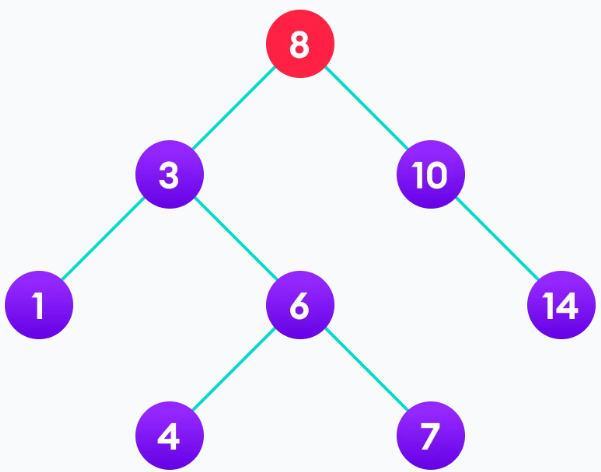
\includegraphics[scale=0.3]{vyhl1.png}
    \end{center}
    }
    \only<3>{
    \begin{center}
        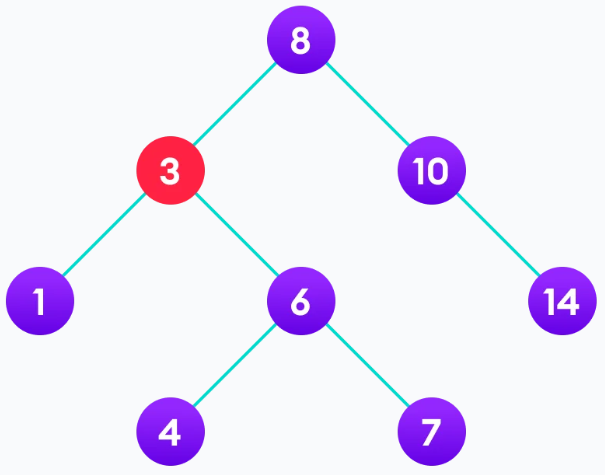
\includegraphics[scale=0.3]{vyhl2.png}
    \end{center}
    }
    \only<4>{
    \begin{center}
        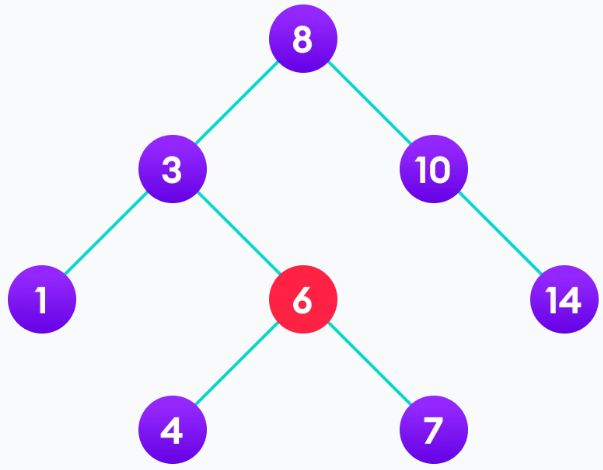
\includegraphics[scale=0.3]{vyhl3.png}
    \end{center}
    }
\end{frame}

\begin{frame}[t]{Vložení klíče}
    \bigskip
    Nový klíč vždy vkládáme na listové úrovni. Hledáme ho pokud nenarazíme na situaci, když nemůžeme jít hlouběji a přidáváme k uzlu nový list.
    \bigskip
    \begin{center}
        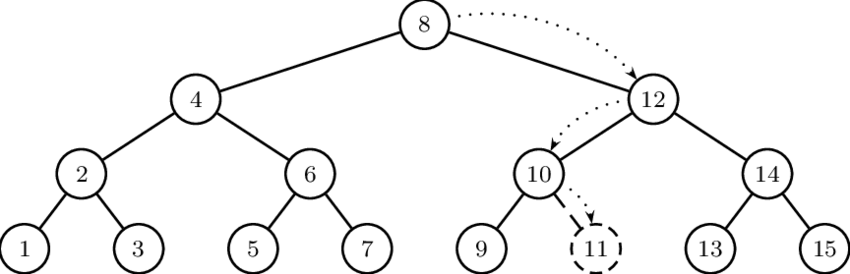
\includegraphics[scale=0.35]{strom.png}
    \end{center}
\end{frame}

\begin{frame}[t]{Smazání klíče}
    Při smazání klíče můžeme se narazit na několik situací:
    \begin{itemize}
        \item Uzel pro smazání je \textbf{listem}\,--\,jednoduše ho mažeme ze stromu.
        \item Uzel pro smazání má \textbf{jedno dítě}\,--\,kopírujeme dítě do uzlu a mažeme dítě.
        \item Uzel pro smazání má \textbf{dvě děti}\,--\,v pravém podstromu uzlu hledáme uzel s nejmenší hodnotou, kopírujeme jeho obsah do původního uzlu a mažeme list. Pokud pravý podstrom neexistuje, děláme to samé s největší hodnotou levého podstromu.
    \end{itemize}
    \medskip
    \begin{center}
        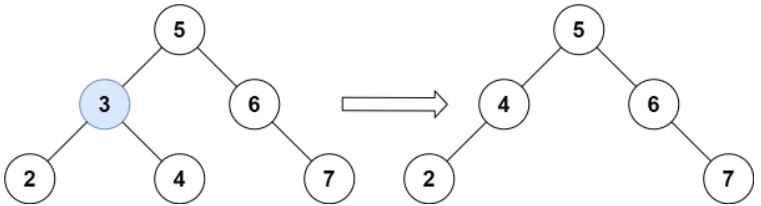
\includegraphics[scale=0.53]{mazani.png}
    \end{center}
\end{frame}

\begin{frame}[fragile]{Pseudokód BST}
    \begin{algorithm}[H]
    \begin{algorithmic}[1]
    \STATE search (value, root) \{
        \IF {(root $==$ NULL)}
            \RETURN NULL;
        \ELSIF{(root.data $==$ value)}
            \RETURN root;
        \ELSIF{(root.data $>$ value)}
            \RETURN search (value, root.left);
        \ELSE
            \RETURN search (value, root.right);
        \ENDIF
    \STATE \}
    \end{algorithmic}
    \caption{Pseudokód pro vyhledávání klíče v BST}
    \label{alg:seq}
    \end{algorithm}
\end{frame}

\begin{frame}{Složitost BST, závěr}
    Operace s BST se provádí rychleji, než s obyčejným polem. Při práci s polem potřebujeme $O(n)$ kroků, kde $n$ je velikost pole.
    
    Pro práci se stromem provádíme $O(h)$ operací, kde $h$ je maximální hloubka stromu. V nejoptimálnějším případě, když hloubka všech listů je stejná, strom má $n=2^{h}-1$ vrcholů, takže $O(h)=O(\log n)$. 
    
    Musíme ale dávat pozor, aby se BST nestal polem. Naštěstí, existují metody optimalizace hloubky stromů pro jejich vybalancování.  
\end{frame}

\begin{frame}{Použité zdroje}
    \begin{thebibliography}{9}
        \bibitem{alg} \href{https://www.algoritmy.net/article/75/Porovnani-algoritmu}{Algoritmy.net: Porovnání řadicích algoritmů}
        
        \bibitem{strukt}
        \href{https://habr.com/ru/post/65617/}{Habr.com: struktury dannych: binarnye derevya}
        
        \bibitem{bst}
        \href{https://www.geeksforgeeks.org/binary-search-tree-data-structure/}{GeeksforGeeks: Binary Search Tree}
        
        \bibitem{bst2}
        \href{https://www.programiz.com/dsa/binary-search-tree}{Programiz: Binary Search Tree}
\end{thebibliography}
\end{frame}

\begin{frame}[standout]
    \huge Děkuji za pozornost!
\end{frame}
\end{document}
